Das Problem der globalen Beleuchtung durch physikalisch basierter Monte-Carlo Integration und gleichzeitiges Erreichen der 
Echtzeitanforderung von 30$\frac{Bilder}{s}$ ist ein bekanntes Problem. Dazugehörige bekannte Lösungsansätze 
ziehen bereits temporale Lösungsansätze z.B. temporales Akkumulieren \cite{schied2017spatiotemporal} in Betracht. 
\par 

Eine klassisches Formulierung \cite{UE4TAA} haben wir beispielhaft wie im Folgenden angewandt:

\begin{algorithm}[H]
    \caption{Beispielhafte Akkumulation}
    \begin{algorithmic}[1]
        \State Texture2D current\_frame;
        \State RWTexture2D accumulation\_buffer;
        \State float4 current\_color = current\_frame[pixel\_pos];
        \State float4 prev\_color = accumulation\_buffer[pixel\_pos];
        \State accumulation\_buffer[pixel\_pos] = 
        \State (frame\_count * prev\_color + current\_color) / (frame\_count + 1);
    \end{algorithmic}
    \label{alg:TemporalAccumulation}
\end{algorithm}

Diese klassische Formulierung, verletzt unsere Annahme für die Quantilfunktion \ref{eq:inverse Funktion}
in den \nameref{ch:Content2:sec:a Posteriori}-Bedingungen des zugrundeliegenden Algorithmus 
\ref{ch:Temporaler Algorithmus}. Denn durch diese Akkumulation bestimmt nicht mehr allein der 
Anfangswert die Pixelfarbe!
\par 

\begin{figure}[H]
    
    \label{subsec:Temporales Projezieren}
\end{figure}
Um die a Posteriori Annahmen anwenden zu können und die Vorbedingungen der Quantilfunktion \ref{eq:inverse Funktion}
für unseren Algorithmus zu erfüllen brauchen wir eine erneute Permutation! Denn durch die Permutation haben wir wieder garantiert, 
dass je ein Anfangswert $x \in [0,1]$ auf je ein Pixelfarbwert abbgebildet wird. Wir nehmen die Idee zur Verbesserung der Zeitkohärenz
aus \cite[S.9/10]{hal02158423} auf. Da unser Algorithmus davon ausgeht, dass zwei aufeinanderfolgende Bilder gleiche Pixelwerte 
besitzen, erhoffen wir uns durch eine temporale Projektion ein Verbesserung bei der \nameref{ch:Content1:sec:blue noise} Verteilung 
falls sich z.B. durch Kamerabewegung die Farbgebung der Pixel zwischen Ihnen ändert. Die temporale Projektion, welche wir hier 
anwenden, baut auf aktuelle verbreitete Techniken des TAA auf \cite{INSIDETAA}.

\begin{figure}[H]
        \centering
        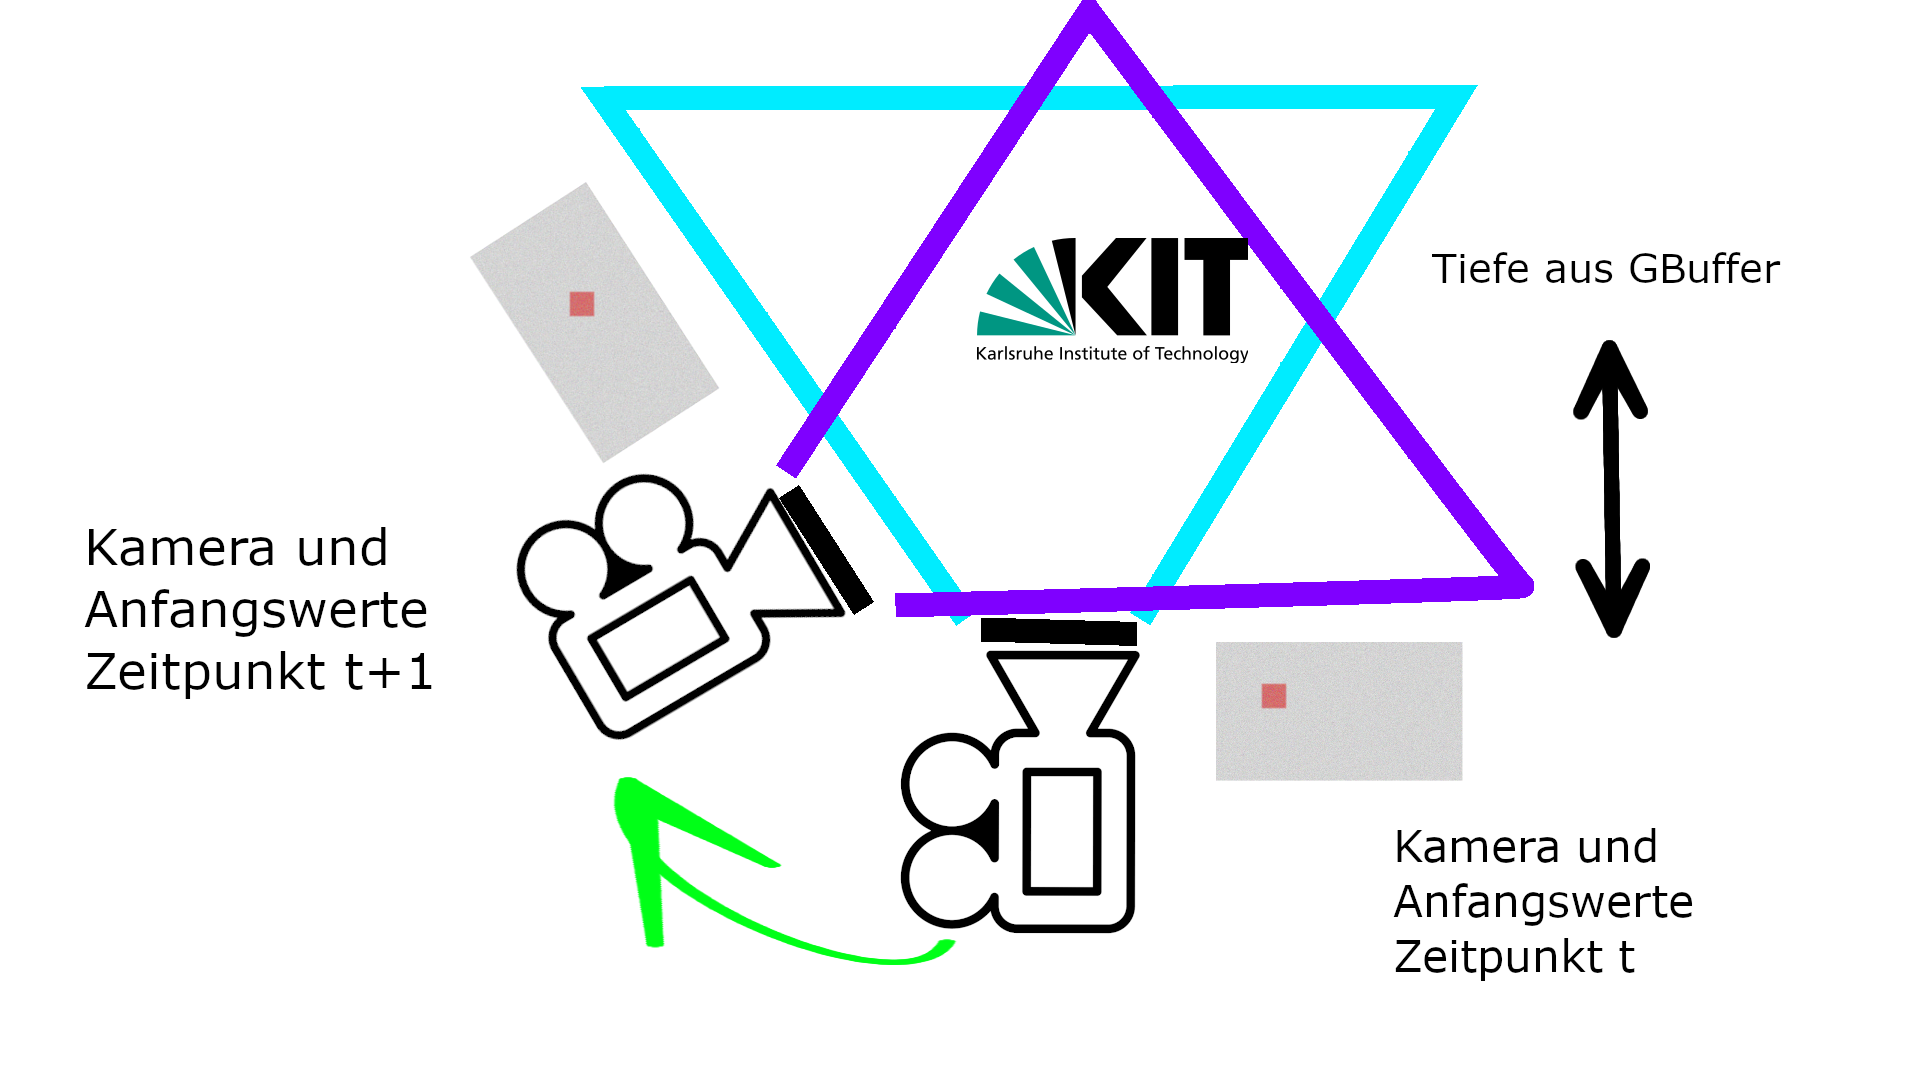
\includegraphics[width=\linewidth]{content/TemporalerAlg/Bilder/Reprojection/TemporalReprojectPrincipal.png}
        \caption{Übersicht Temporal Reprojection}
        \label{pic:Uebersicht_Temporal_Reprojection}
\end{figure}

Wir benutzen die berechneten Tiefenwerte aus dem GBuffer (siehe auch unserer \nameref{pic:Render Graph}) und die jeweiligen 
View-Projektion-Matrizen der Kameras, um herauszufinden welche Koordinaten der jeweilige Anfangswert von Bild t im Bild t+1 
haben würde aufgrund der Drehung.
\par 

